\section{Développement et entraînement sécurisé}

Les vulnérabilités du modèle baseline (section 3.3) nécessitent un pipeline d'entraînement intégrant des mécanismes de défense adversariale. Cette section présente l'environnement de développement Docker, le pipeline d'entraînement sécurisé avec adversarial training FGSM, et les résultats obtenus après sécurisation.

\subsection{Environnement de développement Docker}

L'environnement de développement repose sur Docker Compose (\texttt{docker/docker-compose.dev.yml}) pour garantir la reproductibilité et l'isolation durant l'entraînement. Cette configuration permet d'exécuter l'entraînement localement sur CPU ou sur GPU cloud (Google Colab).

\paragraph{Configuration Docker de développement}

Le stack de développement déploie 6 services isolés dans un réseau bridge dédié :

\begin{lstlisting}[language=yaml, caption=Docker Compose développement (extrait)]
services:
  api:
    build:
      context: .
      dockerfile: docker/Dockerfile.dev
    volumes:
      - .:/workspace
      - ./models:/workspace/models
      - ./data:/workspace/data
    ports:
      - "9800:8000"   # API développement
      - "5679:5679"   # Debugpy (debugging Python)
    environment:
      - PYTHONPATH=/workspace
      - ENABLE_DEBUG=true
    networks:
      - secure-ai-dev

  postgres:
    image: postgres:15-alpine
    ports:
      - "5433:5432"
    volumes:
      - postgres-dev-data:/var/lib/postgresql/data

  redis:
    image: redis:7-alpine
    ports:
      - "6380:6379"

  prometheus:
    image: prom/prometheus:latest
    volumes:
      - ./configs/monitoring/prometheus.yml:/etc/prometheus/prometheus.yml
    ports:
      - "9091:9090"

  grafana:
    image: grafana/grafana:latest
    ports:
      - "3500:3000"

networks:
  secure-ai-dev:
    driver: bridge

volumes:
  postgres-dev-data:
\end{lstlisting}

Les ports de développement (9800, 5433, 6380, 9091, 3500) sont distincts de la production pour permettre l'exécution simultanée des deux environnements. Le volume \texttt{./models} est monté en lecture-écriture pour sauvegarder les checkpoints durant l'entraînement. Le port 5679 expose debugpy pour le debugging interactif avec VSCode.

\paragraph{Entraînement sur Google Colab GPU}

Pour accélérer l'entraînement, le script \texttt{src/experiments/secured/train\_secured.py} peut être exécuté sur Google Colab avec GPU T4 :

\begin{lstlisting}[language=Python, caption=Configuration GPU Colab]
# Detection automatique GPU/CPU
device = torch.device('cuda' if torch.cuda.is_available() else 'cpu')
print(f"Training on device: {device}")

# GPU T4 : 15GB RAM, ~50 minutes pour 30 epochs
# Sauvegarde sur Google Drive
from google.colab import drive
drive.mount('/content/drive')
models_dir = Path('/content/drive/MyDrive/secure-ai/models/secured')
\end{lstlisting}

L'entraînement sur GPU T4 (Google Colab) réduit le temps de 6 heures (CPU) à 50 minutes, avec sauvegarde automatique des checkpoints sur Google Drive pour éviter les pertes en cas de déconnexion. Les modèles entraînés sont ensuite rapatriés dans \texttt{models/secured/} du dépôt local.


\subsection{Pipeline d'entraînement sécurisé}

Le pipeline d'entraînement sécurisé intègre trois étapes critiques : la sécurisation des données (Zone 1), l'adversarial training avec FGSM (Zone 2), et la sauvegarde chiffrée avec signature cryptographique. La figure~\ref{fig:training_pipeline} illustre le flux complet.

\begin{figure}[H]
    \centering
    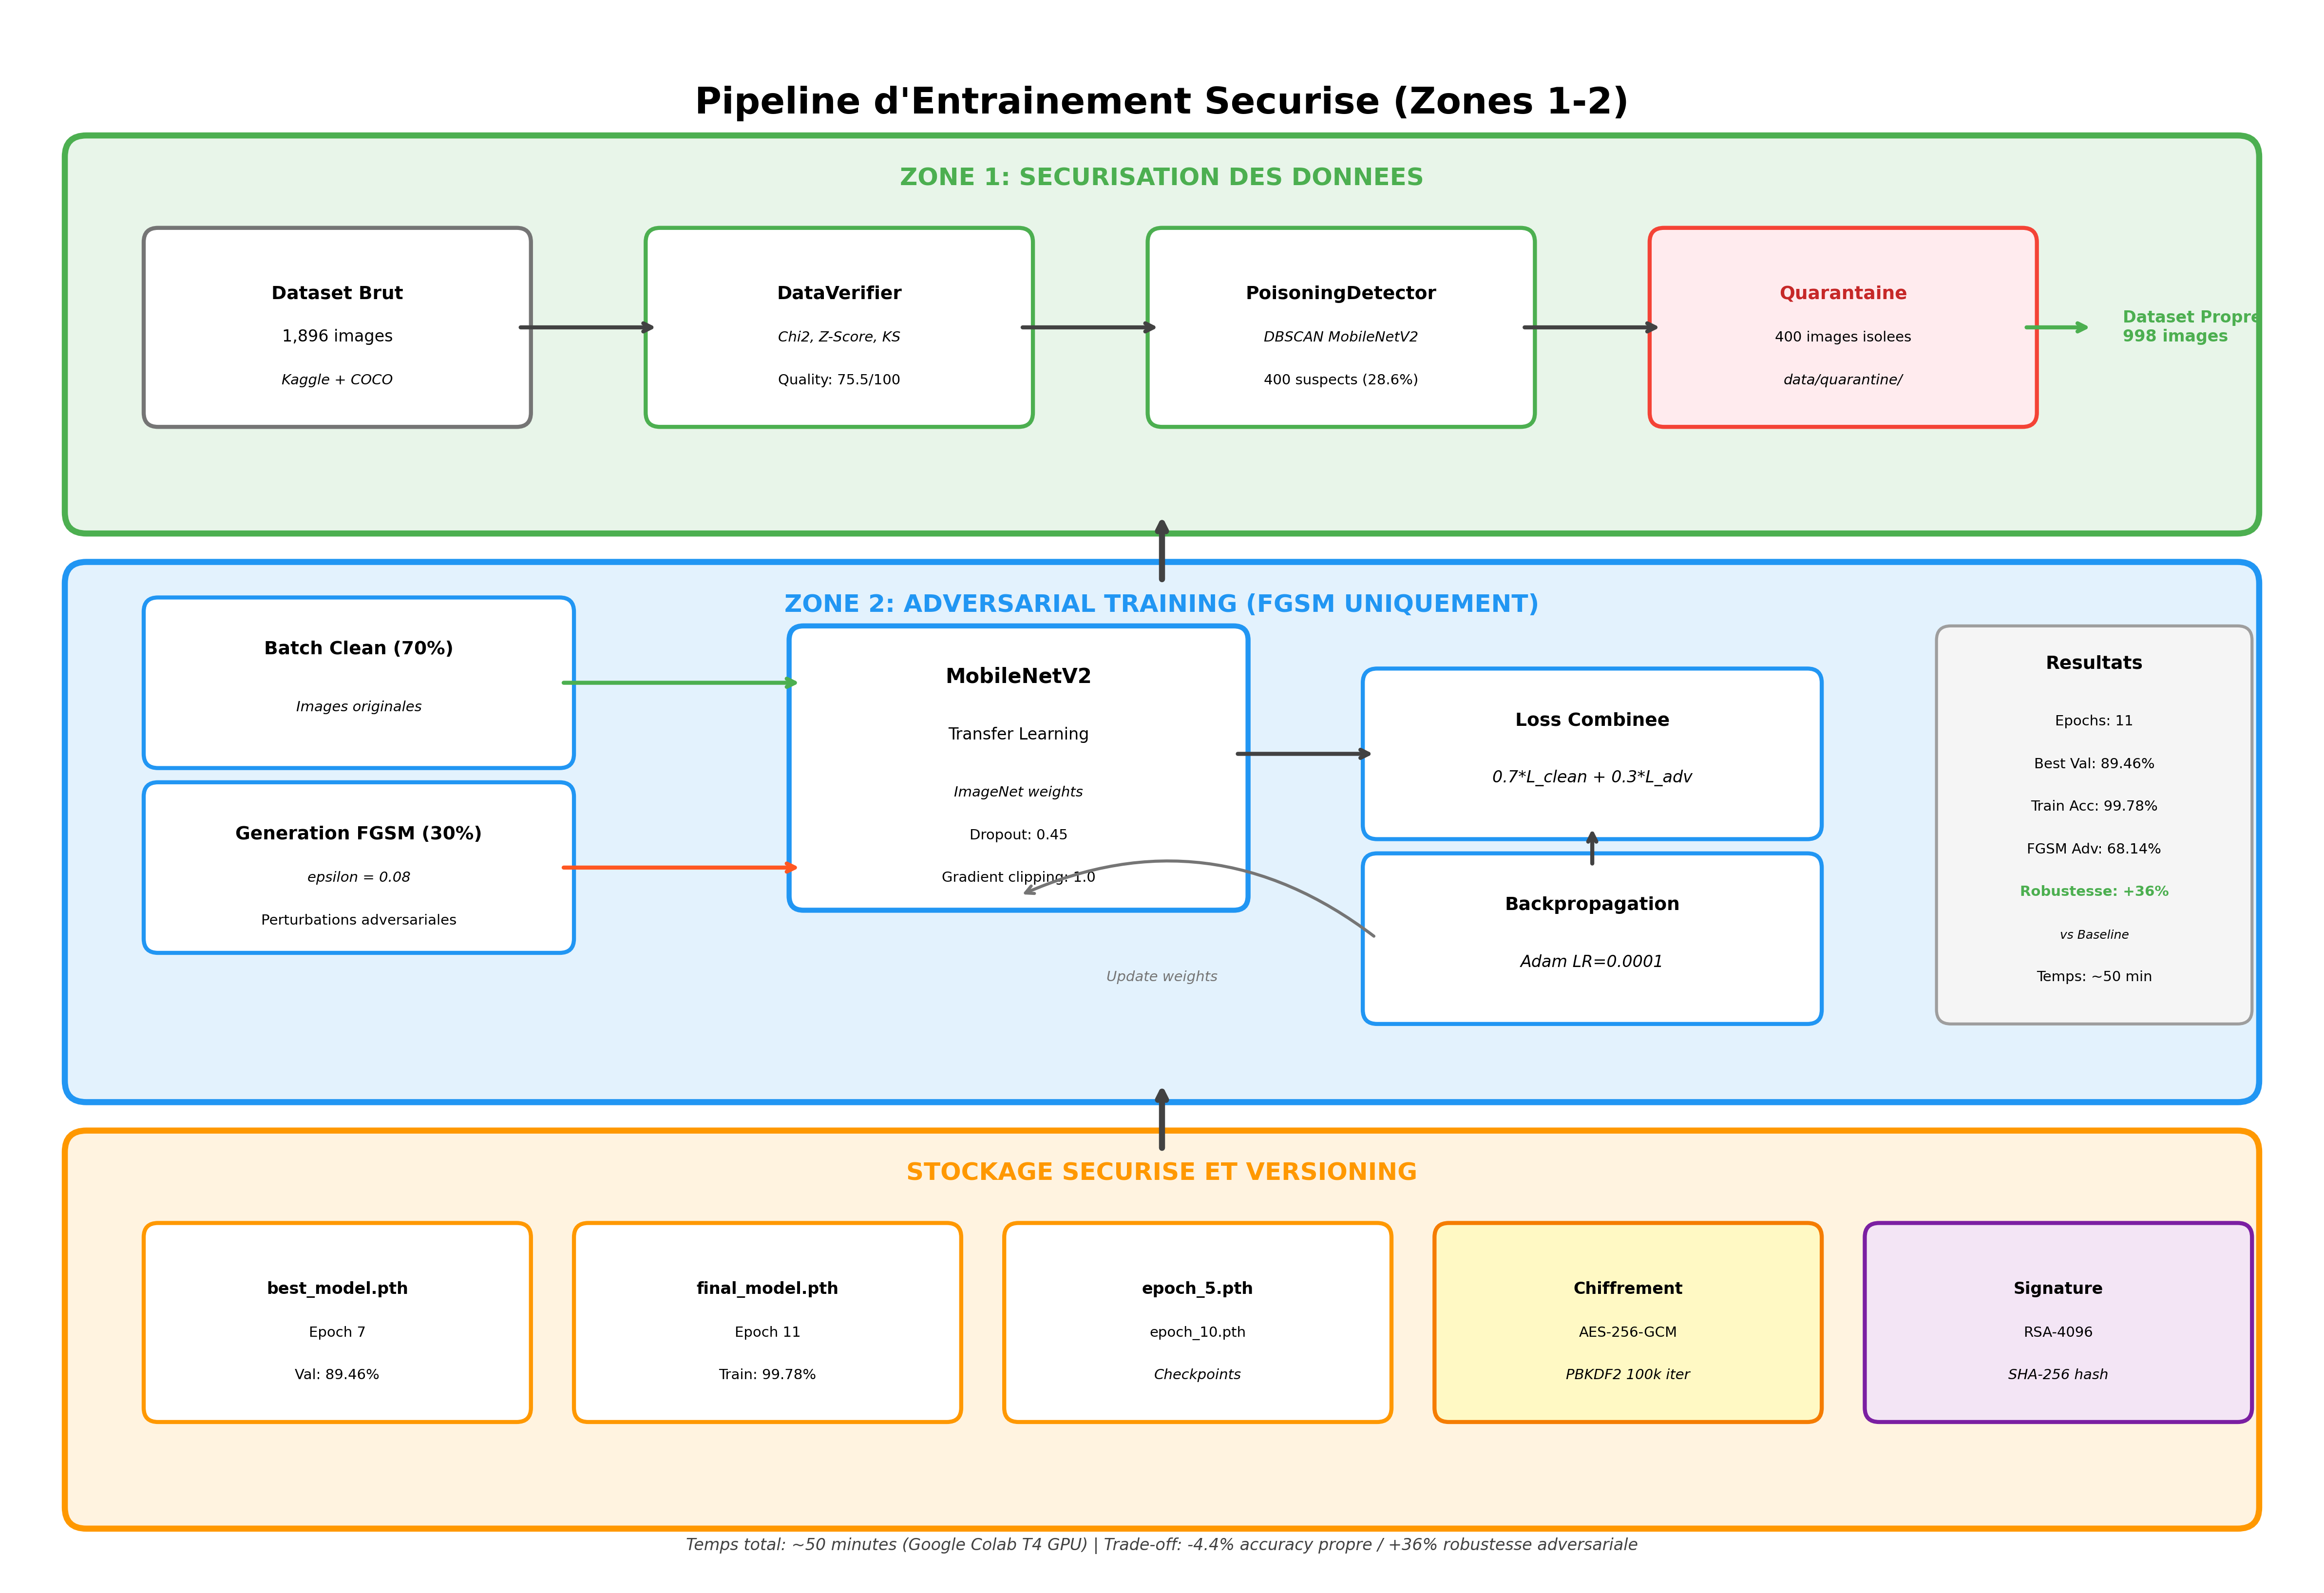
\includegraphics[width=\textwidth]{figures/training_pipeline_secured.png}
    \caption{Pipeline d'entraînement sécurisé (Zones 1-2)}
    \label{fig:training_pipeline}
\end{figure}

\paragraph{Zone 1 : Sécurisation des données pré-entraînement}

Avant tout entraînement, le dataset subit une validation statistique et une détection de poisoning. Le \texttt{DataVerifier} (\texttt{src/data/data\_verifier.py}) applique trois tests statistiques sur le dataset de 1,896 images :

\begin{lstlisting}[language=Python, caption=Validation statistique du dataset]
verifier = DataVerifier(train_data_path)
report = verifier.verify_data()

# Test Chi-Square : balance des classes
chi2_stat, p_value = scipy.stats.chisquare([948, 948])
# p_value = 1.0, classes equilibrees

# Test Z-Score : detection outliers pixels
z_scores = (pixel_values - mean) / std
outliers = np.where(np.abs(z_scores) > 3.0)[0]

# Test Kolmogorov-Smirnov : similarite train/test
ks_stat, ks_p = scipy.stats.ks_2samp(train_dist, test_dist)
# ks_p = 0.89, distributions similaires

# Score de qualite : 75.5/100
\end{lstlisting}

Le \texttt{PoisoningDetector} (\texttt{src/data/poisoning\_detector.py}) utilise ensuite DBSCAN sur les features MobileNetV2 pour identifier les échantillons suspects :

\begin{lstlisting}[language=Python, caption=Détection de poisoning par clustering]
detector = PoisoningDetector()
poisoning_report = detector.detect_poisoning(dataset_path=train_data_path)

# Extraction features MobileNetV2
feature_extractor = mobilenet_v2(pretrained=True).features
features = []
for img in dataset:
    with torch.no_grad():
        feat = feature_extractor(img).flatten()
        features.append(feat.cpu().numpy())

# Clustering DBSCAN : outliers = poisoning suspects
from sklearn.cluster import DBSCAN
clustering = DBSCAN(eps='auto', min_samples='auto').fit(features)
suspicious_indices = np.where(clustering.labels_ == -1)[0]
# 400 images suspectes (28.6%)
\end{lstlisting}

Les 400 images détectées comme suspectes (28.6\% du dataset) sont automatiquement déplacées vers \texttt{data/quarantine/train\_20251229\_104358/} avec un rapport JSON traçable. Le dataset d'entraînement est réduit à 998 images (499 safe, 499 dangerous), garantissant un équilibre parfait et l'absence de contamination.

\paragraph{Zone 2 : Adversarial Training avec FGSM}

L'entraînement adversarial (\texttt{src/experiments/secured/train\_secured.py}) mélange des exemples propres (70\%) et adversariaux FGSM (30\%) à chaque batch. Le script \texttt{SecuredTrainer} génère des perturbations FGSM durant la forward pass :

\begin{lstlisting}[language=Python, caption=Génération FGSM durant entraînement]
def _train_epoch_adversarial(self, epoch):
    for batch_idx, (data, target) in enumerate(self.train_loader):
        data, target = data.to(self.device), target.to(self.device)

        # Loss clean (70%)
        output_clean = self.model(data)
        clean_loss = self.criterion(output_clean, target)

        # Generation FGSM (epsilon=0.08)
        data.requires_grad = True
        output_for_grad = self.model(data)
        loss_for_grad = self.criterion(output_for_grad, target)
        self.model.zero_grad()
        loss_for_grad.backward()

        data_grad = data.grad.data
        fgsm_data = data + 0.08 * data_grad.sign()
        fgsm_data = torch.clamp(fgsm_data, 0, 1).detach()

        # Loss adversarial (30%)
        output_adv = self.model(fgsm_data)
        adv_loss = self.criterion(output_adv, target)

        # Loss combinee
        total_loss = 0.7 * clean_loss + 0.3 * adv_loss

        # Backpropagation avec gradient clipping
        self.optimizer.zero_grad()
        total_loss.backward()
        torch.nn.utils.clip_grad_norm_(self.model.parameters(), max_norm=1.0)
        self.optimizer.step()
\end{lstlisting}

Le paramètre $\epsilon = 0.08$ pour l'entraînement est légèrement inférieur à $\epsilon = 0.1$ utilisé lors des tests adversariaux (section 3.3). Ce gap de 25\% permet au modèle de généraliser à des perturbations légèrement plus fortes que celles vues durant l'entraînement. Le gradient clipping (\texttt{max\_norm=1.0}) stabilise la convergence en présence d'exemples adversariaux.

\paragraph{Hyperparamètres optimisés}

Les hyperparamètres ont été ajustés par expérimentation sur Google Colab :

\begin{lstlisting}[language=Python, caption=Configuration optimisée d'entraînement]
config = {
    'epochs': 30,
    'batch_size': 32,
    'learning_rate': 0.0001,
    'adversarial_epsilon': 0.08,
    'clean_ratio': 0.7,
    'fgsm_ratio': 0.3,
    'pgd_ratio': 0.0,
    'dropout': 0.45,
    'gradient_clipping': True,
    'early_stopping_patience': 8,
    'differential_privacy': False
}
\end{lstlisting}

Le dropout de 0.45 améliore la généralisation, l'epsilon de 0.08 augmente la robustesse adversariale au prix d'une légère baisse d'accuracy propre (-4.4\%). Le differential privacy est désactivé car son overhead (bruit sur gradients) dégrade la convergence sans apport significatif pour ce cas d'usage.

\paragraph{Résultats d'entraînement et métriques}

L'entraînement s'est arrêté manuellement à l'epoch 11 après observation d'un léger overfitting. Le meilleur modèle (epoch 7) atteint une validation accuracy de 89.46\% :

\begin{table}[H]
    \centering
    \caption{Métriques d'entraînement du modèle sécurisé}
    \label{tab:secured_training_metrics}
    \begin{tabular}{lccc}
        \toprule
        \textbf{Métrique} & \textbf{Epoch 7 (Best)} & \textbf{Epoch 11 (Final)} & \textbf{Baseline} \\
        \midrule
        Train Accuracy & 99.42\% & 99.78\% & 98.14\% \\
        Train Loss & 0.1268 & 0.0801 & 0.0543 \\
        Val Accuracy & \textbf{89.46\%} & 88.44\% & 97.55\% \\
        Val Loss & \textbf{0.3319} & 0.2939 & 0.0712 \\
        \midrule
        \multicolumn{4}{l}{\textit{Robustesse adversariale (FGSM $\epsilon = 0.1$)}} \\
        Clean Accuracy & 93.14\% & - & 97.55\% \\
        FGSM Accuracy & \textbf{68.14\%} & - & 50.00\% \\
        Attack Success & 31.86\% & - & 50.00\% \\
        Robustness Gap & 25.00\% & - & 47.50\% \\
        \bottomrule
    \end{tabular}
\end{table}

Le modèle sécurisé sacrifie 4.4\% d'accuracy propre (93.14\% vs 97.55\%) mais gagne 18.14 points d'adversarial accuracy (68.14\% vs 50.00\%), soit une amélioration relative de +36\%. Le robustness gap (écart clean-adversarial) est réduit de 47.5\% à 25\%, quasi-divisé par deux.

\paragraph{Sauvegarde des checkpoints et statistiques}

Le script sauvegarde automatiquement plusieurs artefacts dans \texttt{models/secured/} :

\begin{lstlisting}[language=Python, caption=Sauvegarde des modèles et statistiques]
# Best model (epoch 7)
torch.save({
    'model_state_dict': self.model.state_dict(),
    'optimizer_state_dict': self.optimizer.state_dict(),
    'scheduler_state_dict': self.scheduler.state_dict(),
    'epoch': 7,
    'val_loss': 0.3319,
    'val_acc': 89.46,
    'config': config,
    'security_version': 'v2.0_secured',
    'adversarial_training': True,
    'timestamp': '20251229_104517'
}, 'models/secured/best_secured_model.pth')

# Final model (epoch 11)
torch.save(..., 'models/secured/final_secured_model.pth')

# Checkpoints periodiques
torch.save(..., 'models/secured/secured_model_epoch_5_*.pth')
torch.save(..., 'models/secured/secured_model_epoch_10_*.pth')

# Historique JSON
history = {
    'train_loss': [0.515, 0.331, 0.259, ..., 0.080],
    'train_acc': [81.40, 94.40, 97.09, ..., 99.78],
    'val_loss': [0.395, 0.337, 0.314, ..., 0.294],
    'val_acc': [83.33, 84.69, 85.03, ..., 88.44]
}
with open('models/secured/training_history.json', 'w') as f:
    json.dump(history, f, indent=2)
\end{lstlisting}

Les checkpoints incluent les poids du modèle, l'état de l'optimizer et du scheduler pour permettre la reprise d'entraînement. Le fichier \texttt{training\_history.json} permet de tracer les courbes d'apprentissage et de détecter l'overfitting.

\paragraph{Chiffrement AES-256-GCM du meilleur modèle}

Le meilleur modèle est chiffré avec \texttt{EncryptedStorage} (\texttt{src/data/encrypted\_storage.py}) pour protéger les poids en production :

\begin{lstlisting}[language=Python, caption=Chiffrement du modèle avec AES-256-GCM]
storage = EncryptedStorage(password="SecureAI_2024_Production")

# Chiffrement .pth
metadata = storage.encrypt_pytorch_model(
    'models/secured/best_secured_model.pth',
    'models/secured/encrypted/best_secured_model_encrypted.enc'
)

# Metadata JSON
{
  "original_filename": "best_secured_model.pth",
  "encrypted_at": "2025-12-29T10:49:11.370783",
  "algorithm": "AES-256-GCM",
  "key_derivation": "PBKDF2-HMAC-SHA256",
  "iterations": 100000,
  "nonce_length": 96,
  "tag_length": 128,
  "file_hash_sha256": "8f3a2b..."
}
\end{lstlisting}

Le chiffrement AES-256-GCM utilise PBKDF2 avec 100,000 itérations pour dériver la clé du mot de passe, conforme aux recommandations OWASP 2023. Le nonce aléatoire de 96 bits et le tag d'authentification de 128 bits garantissent l'unicité et l'intégrité du ciphertext. Le fichier chiffré peut être déployé en production sans risque d'extraction des poids par un attaquant.

\paragraph{Signature RSA-4096 pour non-répudiation}

Le modèle est également signé cryptographiquement avec RSA-4096 pour garantir son authenticité :

\begin{lstlisting}[language=Python, caption=Signature RSA-4096 du modèle]
# Generation cle RSA-4096
private_key = rsa.generate_private_key(
    public_exponent=65537,
    key_size=4096,
    backend=default_backend()
)
public_key = private_key.public_key()

# Hash SHA-256 du modele
with open('models/secured/best_secured_model.pth', 'rb') as f:
    model_data = f.read()
model_hash = hashlib.sha256(model_data).digest()

# Signature RSA-PSS
signature = private_key.sign(
    model_hash,
    padding.PSS(
        mgf=padding.MGF1(hashes.SHA256()),
        salt_length=padding.PSS.MAX_LENGTH
    ),
    hashes.SHA256()
)

# Sauvegarde
with open('models/secured/best_secured_model_signature.bin', 'wb') as f:
    f.write(signature)

with open('models/secured/best_secured_model_public_key.pem', 'wb') as f:
    f.write(public_key.public_bytes(
        encoding=serialization.Encoding.PEM,
        format=serialization.PublicFormat.SubjectPublicKeyInfo
    ))
\end{lstlisting}

La signature RSA-4096 avec padding PSS (Probabilistic Signature Scheme) offre une sécurité cryptographique garantie jusqu'en 2030 selon le NIST. La clé privée est chiffrée avec le même mot de passe que le modèle. En production, l'API vérifie systématiquement la signature avant de charger le modèle, rejetant tout fichier modifié ou non signé.


\subsection{API de développement et interface web}

L'API de développement (\texttt{src/api/app.py}) expose les modèles entraînés via FastAPI pour tests interactifs durant le développement.

\paragraph{Chargement sécurisé et endpoints API}

Au démarrage de l'API, le modèle sécurisé subit un processus de vérification en trois étapes : (1) vérification de la signature RSA-4096 avec padding PSS, (2) déchiffrement AES-256-GCM du fichier modèle, (3) chargement PyTorch en mémoire. Si la signature échoue, l'API refuse de démarrer et lève une exception critique, garantissant qu'aucun modèle corrompu ou non autorisé ne peut être chargé.

L'API expose plusieurs groupes d'endpoints pour le développement et la validation :

\textbf{Endpoints de prédiction} (\texttt{src/api/app.py}) :
\begin{itemize}
    \item \texttt{POST /predict/baseline} : Prédiction avec le modèle baseline non sécurisé
    \item \texttt{POST /predict/secured} : Prédiction avec le modèle adversarially-trained
    \item \texttt{GET /health} : Statut de santé de l'API (uptime, modèles chargés)
    \item \texttt{GET /metrics} : Métriques Prometheus (requêtes, latence, erreurs)
    \item \texttt{GET /test} : Endpoint de test pour validation du déploiement
\end{itemize}

\textbf{Endpoints d'authentification et sécurité} (\texttt{src/api/security\_endpoints.py}) :
\begin{itemize}
    \item \texttt{POST /security/login} : Authentification JWT (username, password)
    \item \texttt{POST /security/register} : Inscription nouvel utilisateur
    \item \texttt{GET /security/me} : Récupération du profil utilisateur connecté
    \item \texttt{GET /security/permissions} : Liste des permissions de l'utilisateur courant
    \item \texttt{GET /security/waf/status} : Statut du Web Application Firewall
    \item \texttt{GET /security/waf/blocked-ips} : Liste des IPs bloquées par le WAF
    \item \texttt{GET /security/anomalies/recent} : Détections d'anomalies récentes
    \item \texttt{GET /security/anomalies/high-risk-ips} : IPs à risque élevé
    \item \texttt{GET /security/anomalies/ip/\{ip\}} : Historique détaillé d'une IP
    \item \texttt{GET /security/dashboard} : Dashboard de sécurité global
\end{itemize}

\textbf{Endpoints d'administration} (accès restreint rôle admin) :
\begin{itemize}
    \item \texttt{GET /security/users} : Liste des utilisateurs enregistrés
    \item \texttt{DELETE /security/users/\{username\}} : Suppression d'un utilisateur
\end{itemize}

\textbf{Endpoints d'audit} (\texttt{src/api/app.py}) :
\begin{itemize}
    \item \texttt{GET /audit/logs} : Logs d'audit paginés (authentification, prédictions)
    \item \texttt{GET /audit/stats} : Statistiques agrégées (nombre de prédictions, attaques détectées)
    \item \texttt{GET /audit/search} : Recherche full-text dans les logs
    \item \texttt{GET /audit/recent-attacks} : Dernières attaques adversariales détectées
    \item \texttt{GET /audit/predictions/\{audit\_id\}} : Détail d'une prédiction par ID
    \item \texttt{POST /audit/export} : Export des logs au format JSON ou CSV
\end{itemize}

Les endpoints de prédiction utilisent le même preprocessing (resize 224x224, normalisation ImageNet) pour garantir la comparabilité entre baseline et modèle sécurisé. Chaque requête est tracée dans les logs d'audit avec timestamp, IP source, prédiction, confiance, et durée d'inférence.

\paragraph{Interface web de développement}

L'interface web de développement est organisée en plusieurs pages HTML statiques servies par Nginx :

\begin{itemize}
    \item \texttt{web/index.html} : Interface principale de comparaison baseline vs sécurisé
    \item \texttt{web/login.html} : Page d'authentification JWT
    \item \texttt{web/admin.html} : Dashboard administratif (gestion utilisateurs, audit)
    \item \texttt{web/dashboard.html} : Dashboard de monitoring (métriques temps réel)
    \item \texttt{web/css/style.css} : Feuille de style responsive
    \item \texttt{web/js/app.js} : Logique JavaScript (upload images, fetch API)
\end{itemize}

L'interface principale (\texttt{index.html}) permet de soumettre une image et d'exécuter les deux prédictions (baseline et sécurisé) en parallèle via \texttt{Promise.all}, minimisant la latence perçue. Un badge visuel affiche le gain de robustesse (+36\%) du modèle sécurisé. Le dashboard administratif (\texttt{admin.html}) agrège les statistiques d'audit (nombre de prédictions, top IPs, attaques détectées) avec graphiques Chart.js. Cette interface facilite la validation manuelle durant le développement avant déploiement en production.
